\documentclass{sj_surrey_article}
\usepackage{graphicx}
\usepackage[margin=1.5cm]{geometry}
% Write the approved title of your dissertation
\title{Reinforcemnt Learning in Pokémon Red to explore complex multi-reward environments}

% Write your full name, as in University records
\author{Liam O'Driscoll, 6640106}

% Write the month and year of your submission
\date{ [FILL THIS IN BEFORE SUBMISSION] XX November 2023}

% Uncomment the line for the Degree you are registered for
\degree{Bachelor of Science in Computer Science with a year in placement}

% Write the full name of your supervisor, without any titles
\supervisor{Sotiris Moschoyiannis}

\begin{document}
\maketitle



\section{Introduction}
This section should contain an introduction to the problem aims and objectives (0.5 page)
\subsection{Aims}
Here you need to include the aims
\begin{itemize}
\item aim one goes here
\item aim two goes here
\end{itemize}

This setup is av
\subsection{Objectives}
Here you need to include the objectives
\begin{itemize}
\item objective one goes here
\item objective two goes here
\end{itemize}

\section{Literature Review}
1 page of background and literature review. Here you will need to references things. Gamal et al.~\cite{gamal} introduce the concept of \ldots

\section{Technical overview}
1 page of overview. My approach is shown in Figure~\ref{fig:sample}. You can draw the diagram in powerpoint and save the picture

\begin{figure}[thp]
   \begin{center}
         \scalebox{0.5}{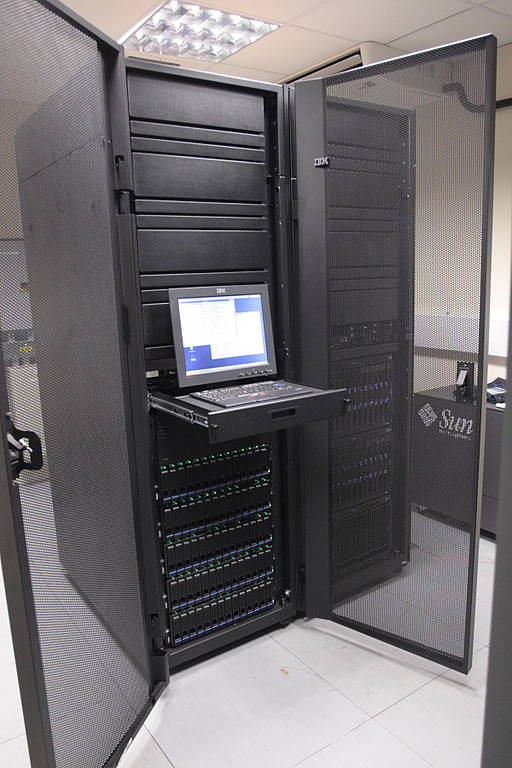
\includegraphics[width=0.8\textwidth]{Figures/tempest}}
   \end{center}
   \caption{An example figure}
   \label{fig:sample}
\end{figure}

\section{Workplan}
The following work plan is what I will be using for the project is shown in Figure~\ref{fig:sample2}.

\begin{figure}[thp]
   \begin{center}
         \scalebox{0.5}{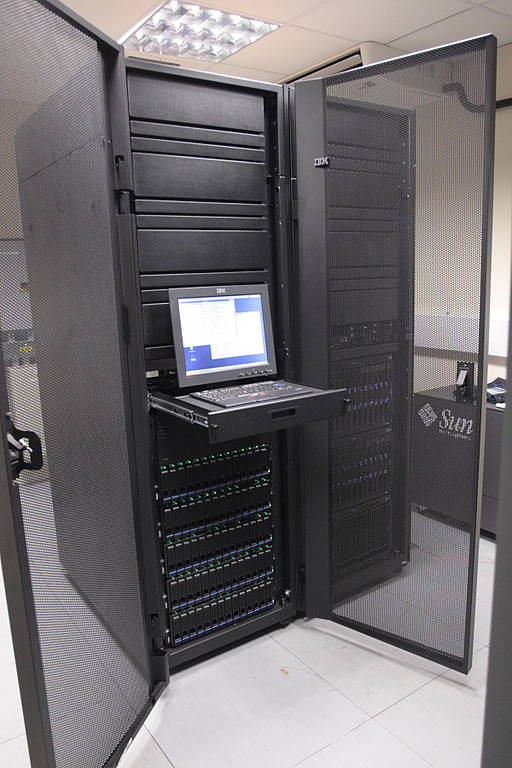
\includegraphics[width=0.8\textwidth]{Figures/tempest}}
   \end{center}
   \caption{Another example figure}
   \label{fig:sample2}
\end{figure}

% appendices
\appendix
%\include{appenda}
%\include{appendb}

\bibliographystyle{IEEEtran}
\bibliography{references}

\end{document}
